% =================================================================================================
% File:			gest_recipe.tex
% Description:	Defiinisce la sezione relativa ad un capitolo del documento
% Created:		2015-04-21
% Author:		Tesser Paolo
% Email:		tesser.paolo@mashup-unipd.it
% =================================================================================================
% Modification History:
% Version		Modifier Date		Change											Author
% 0.0.1 		2015-04-21 			creato scheletro doc							Tesser Paolo
% =================================================================================================
%

% CONTENUTO DEL CAPITOLO
\section{Gestione delle Recipe} % (fold)
\label{sec:gestione_delle_recipe}


	\subsection{Contenuti Sezione} % (fold)
	\label{sub:contenuti_sezione}
		All'utente amministratore sono concessi permessi di modifica e gestione delle recipe\gloss{}.
		La gestione prevede:
		\begin{itemize}
			\item Aggiunta di una nuova recipe\gloss{};
			\item Eliminazione di una o più recipe\gloss{};
			\item Visualizzazione classifica delle recipe\gloss{};
		\end{itemize}


	\subsection{Aggiunta di una nuova recipe}
		Dal menu principale situato nella dashboard\gloss{} del sistema è possibile visualizzare l'elenco delle recipe\gloss{} premendo sull'apposito pulsante \textbf{Recipe}.\newline
		Tramite il pulsante \textbf{New Recipe} è possibile accedere alla nuova pagina (Figura: \ref{fig:aggiunta_nuova_recipe}) per l'inserimento guidato di nuove recipe\gloss{}.
		\begin{figure}[H]
			\centering
			\centerline{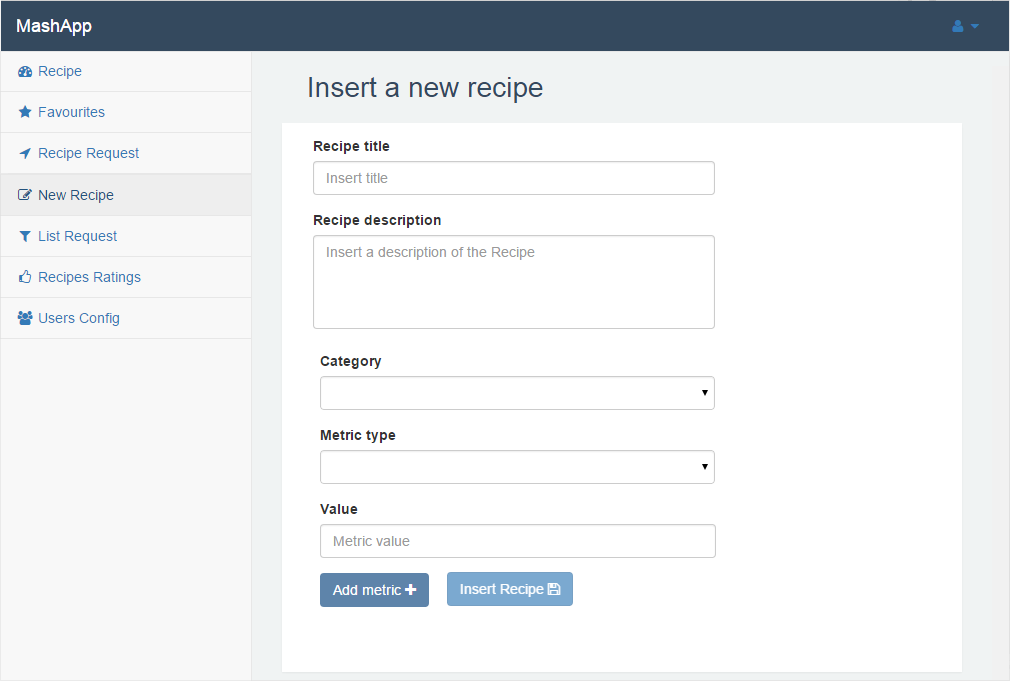
\includegraphics[width=14cm]{images/nuova_ricetta.png}}
			\caption{Aggiunta nuova recipe}
			\label{fig:aggiunta_nuova_recipe}
		\end{figure}
		Per aggiungere una nuova nuova recipe\gloss{} è necessario compilare tutti i campi del form\gloss{} (Figura: \ref{fig:aggiunta_nuova_recipe}) con i seguenti dati:
		\begin{itemize}
			\item Nome della recipe;
			\item Descrizione della recipe;
			\item Parametri relativi alla recipe dipendenti dal/dai social network di interesse;
		\end{itemize}
		È possibile selezionare uno o più social network e uno o più parametri per ciascuna selezione.\newline
		Al termine della procedura guidata è necessario premere il pulsante di \textbf{Insert Recipe} per salvare le modifiche ed aggiungere così la recipe\gloss{} al sistema.
	% END


	\subsection{Eliminazione Recipe}
		L'amministratore può eliminare una recipe\gloss{} e tutti i dati ad essa associati dal sistema.\newline
		Per accedere all'area dedicata della dashboard\gloss{} si deve premere sul pulsante \textbf{Recipe}\gloss{}. Dall'elenco delle recipe\gloss{} (Figura: \ref{fig:dashboard}) è disponibile il pulsante \textbf{Delete recipe}.
		L'eliminazione della recipe è istantanea si può così procedere ad una nuova operazione.
	% END

	
	\subsection{Visualizzazione classifica recipe}
		L'utente amministratore può visualizzare la classifica (Figura: \ref{fig:votazioni_ricette}) delle recipe\gloss{} in ordine dalla più apprezzata alla meno apprezzata.\newline
		Per accedere alla sezione è richiesto di premere l'apposito pulsante \textbf{Recipes Ratings} dal menu principale nella dashboard\gloss{}.\newline
		\begin{figure}[H]
			\centering
			\centerline{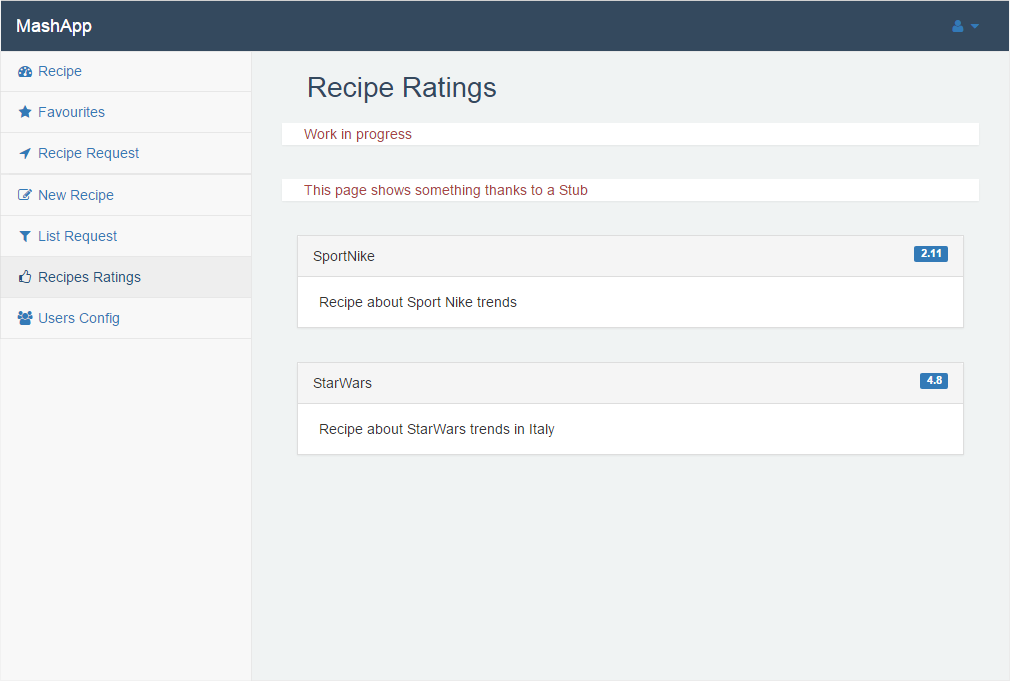
\includegraphics[width=14cm]{images/votazioni_ricette.png}}
			\caption{Punteggi recipes}
			\label{fig:votazioni_ricette}
		\end{figure}
		Nel caso in cui nessun utente abbia ancora dato un giudizio sulle recipe presenti nel sistema, la classifica risulterà vuota.\newline
		Un messaggio avviserà l'utente amministratore se questa situazione dovesse verificarsi.
	% END


% section Gestione delle Recipe (end)